%!TEX TS-program = lualatex
\documentclass[]{friggeri-cv}
\usepackage{afterpage}
\usepackage{hyperref}
\usepackage{color}
\usepackage{xcolor}
\hypersetup{
    pdftitle={},
    pdfauthor={},
    pdfsubject={},
    pdfkeywords={},
    colorlinks=false,       % no lik border color
   allbordercolors=white    % white border color for all
}
\addbibresource{bibliography.bib}
\RequirePackage{xcolor}
\definecolor{pblue}{HTML}{0395DE}

\begin{document}
\header{Arshpreet}     {Singh}
      {Senior Software Engineer}

% Fake text to add separator
\fcolorbox{white}{gray}{\parbox{\dimexpr\textwidth-2\fboxsep-2\fboxrule}{%
.....
}}

% In the aside, each new line forces a line break
\begin{aside}
  \section{Address}
    3159, Sec-40D
    Chandigarh,Punjab, India
    ~
  \section{Tel \& LinkedIn}
    +91 991 5959387
    \href{http://www.linkedin.com/in/arsh840/}{www.linkedin\\.com/in/arsh840/}
    \href{https://stackoverflow.com/users/1540739/arshpreet}{www.stackoverflow\\.com/in/arshpreet/}
    ~
  \section{Mail}
    \href{mailto:arsh840@gmail.com}{\textbf{arsh840@}\\gmail.com}
    ~
  \section{Web \& Git}
    \href{http://www.arshpreetsingh.wordpress.com}{arshpreetsingh.wordpress\\.com}
    \href{https://medium.com/@arshpreetsingh}{https://medium.com/@arshpreet\\singh}
    \href{https://github.com/arshpreetsingh}{github.com/arshpreet\\singh}
    ~
  \section{Programming}
    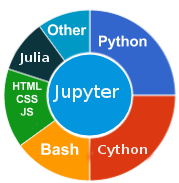
\includegraphics[scale=0.62]{img/programming.png}
    ~
  \section{OS Preference}
    \textbf{GNU/Linux}
\includegraphics[scale=0.40]{img/5stars.png}
    \textbf{Unix}
\includegraphics[scale=0.40]{img/5stars.png}
    \textbf{MacOS}
\includegraphics[scale=0.40]{img/5stars.png}
    \textbf{Windows}
\includegraphics[scale=0.40]{img/2stars.png}
    ~
  \section{Personal Skills}
    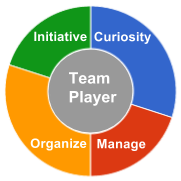
\includegraphics[scale=0.62]{img/personal.png}
    ~
\end{aside}

\section{Experience}
\begin{entrylist}
  \entry
  {04/20 - Now }
  {Lead Engineer}
  {ITC India, Bangalore}
  {Technology Stack: Python, Docker, Go-lang and Jenkins. Leading team of four Engineers to deal with Data Operations and Production bugs related to Trading-Systems. Responsible for code evalutions, UnitTests,
  Integration Testing, dealing with Data-Processing pipelines.}
  \entry
    {01/19 - 04/20 }
    {Senior Software Engineer}
    {Maropost India, Chandigarh}
    {Micro-Services Development and Deployment using Technology Stack: Go-lang, Protocol Buffers, Kafka, Docker, Kuber-netes and Rancher. Responsible for Manneging GCP and Infrastructure
    for High Availability, Replaced RoR Services with GoLang to improve efficiency of Platform, Solely responsible to implement containerization for various projects.}
   \entry
    {08/17 - 04/18}
    {Senior Software Engineer}
    {Netsmartz Chandigarh}
    {Development and Deployment of MicroServices using Technology Stack: Python, Flask, Docker. Development of in-house framework to achieve Periodic Automation Testing for complete platform,
    Worked on BlockChain Project using Hyperledger.}
  \entry
    {05/16 - 08/17}
    {Full-Stack Python Developer}
    {RevInfotech Ludhiana}
    {Design and development of Software Projects, Active participation with clients to understand business needs and Producing End to End Solutions using Python Stack. Single handedly worked on Full Stack
    Python projects from Development to Deployment over Cloud, Developed Automated Crypto Trading bots by enhancing the power of Machine-Learning.\\}
    \entry
    {01/14 - 04/16}
    {Web Developer}
    {FutureTech IT centre Ludhiana}
    {Developed various projects using technologies HTML, CSS, JavaScript, Python, C and shell Script.\\}
    \entry
    {01/13 - 06/13}
    {Industrial Training}
    {SysInfocom, Chandigarh}
    {Training for Linux Desktop and Server Administration, management and migration of servers.\\}
    \entry
    {06/11 - 07/11}
    {Industrial Training}
    {TCC GNDEC Ludhiana}
    {Worked on college souvenir(Django Based Project).SageMath Deployment on Server and introduced SageMath.\\}
\end{entrylist}
\section{Education}
\begin{entrylist}
  \entry
    {2009 - 2013}
    {Bachelor's Degree in Information Technology}
    {GNDCE Ludhiana,Punjab,India}
    {\emph{}}
  \entry
    {2007 - 2009}
    {Senior Secondary School}
    {DC Model, Ferozepur, India}
    {\emph{}}
\end{entrylist}
\section{Certifications}
\begin{entrylist}
  \entry
    {07/2019}
    {Go Programming Specialization}
    {Coursera}
    {\emph{}}
  \entry
    {05/2019}
    {Ultimate Go Programming}
    {O'Reilly School of Technology}
    {\emph{}}
  \entry
    {11/2018}
    {Julia Scientific Programming}
    {Coursera}
    {\emph{}}
  \entry
    {09/2018}
    {Deep Learning Specialization}
    {Coursera}
    {\emph{}}
  \entry
    {06/2018}
    {Julia Programming for Scientific Computing}
    {Coursera}
    {\emph{}}
  \entry
    {06/2018}
    {BlockChain Basics and Beyond}
    {Lynda.com}
    {\emph{}}
  \entry
    {12/2016}
    {Python for DataScience and Machine Learning}
    {Udemy. E-learning}
    {\emph{}}
\end{entrylist}
\section{Projects}
\begin{entrylist}
\entry
   {02/2020}
   {Transactional Email System}
   {Netsmartz Inc.}
   {\emph{Lead Developer for Transactional Email System built Using Go-lang, Kafka, Docker and Kubernetes}}
\entry
   {10/2019}
   {Deployment Automations}
   {Maropost}
   {\emph{Automation and Optimization of Deployment using Container-Based technologies for Rails Based Project.}}
\entry
   {10/2017}
   {SDN based MicroServices}
   {Netsmartz}
   {\emph{Developed back-end and front-end components of the SDN based technologies for https://www.telstra.com.au/}}
 \entry
    {08/2016}
    {Bitcoin Live Trading using ANN}
    {Revinfotech Ludhiana}
    {\emph{Bitcoin Live Trading is Web-Based System developed Using Django Framework.}}
  \entry
    {12/2015}
    {Gmail Analyser}
    {FutureTech}
    {\emph{Gmail Analyser is Flask Based Solution which provides data of All Emails
as per the request.}}
  \entry
    {03/2016}
    {ParaView Advanced Volume Filter}
    {FutureTech}
    {\emph{ParaView is an open-source, multi-platform data analysis and visualization
application.}}
\end{entrylist}
\begin{aside}

   \section{Languages}
    \textbf{English}
\includegraphics[scale=0.40]{img/4stars.png}
    \textbf{Hindi}
\includegraphics[scale=0.40]{img/5stars.png}
    \textbf{Punjabi}
\includegraphics[scale=0.40]{img/5stars.png}
\end{aside}
\section{Open-Source Contributions}
\begin{entrylist}
 \entry
    {03/2016}
    {Tuxblocks}
    {Github}
    {\emph{Contributed as Developer for Kids4Kids(https://github.com/tux4kids).}}

 \entry
    {03/2016}
    {Open Street Mapping}
    {osm.org}
    {\emph{Contributed to Digital Maps.}}

 \entry
    {03/2016}
    {Browser-Based File-Manager}
    {Github}
    {\emph{Flask based File Manager.}}

 \entry
    {03/2016}
    {Text-to-mp3 Android implementation}
    {Github}
    {\emph{Contributed to Open-source project Plyer and Kivy(https://kivy.org).}}

\end{entrylist}
\begin{flushleft}
\emph{February 11th, 2020}
\end{flushleft}
\begin{flushright}
\emph{Arshpreet Singh Khangura}
\end{flushright}
\clearpage
\end{document}
